\documentclass[11pt]{article} % font size
\usepackage{graphicx}
\usepackage[usenames, dvipsnames]{color}
\usepackage{url}
\usepackage{bbm}
\usepackage{setspace}
\usepackage{amssymb}
\usepackage{amsfonts}
\usepackage{amsmath}
\usepackage{amsthm}
\usepackage{rotating}
\usepackage{harvard}
\usepackage{enumitem}
\usepackage{filecontents}
\usepackage{verbatim}
\usepackage{subfiles}
\usepackage{csvsimple}
\usepackage{pdflscape}
\usepackage{longtable}
\usepackage{listings}
\usepackage[utf8]{inputenc} % package for nonstandard letters (umlauts etc)
\usepackage{natbib} % bibliography
\usepackage{booktabs} % For nice tables
% setting up the design
\usepackage[paper=a4paper,left=30mm,right=30mm,top=30mm,bottom=30mm]{geometry}
\renewcommand{\baselinestretch}{1.5} % line spacing
\renewcommand{\topfraction}{0.99}
\renewcommand{\bottomfraction}{0.99}
\renewcommand{\textfraction}{0.01}
\renewcommand{\floatpagefraction}{0.99}
\setlength{\footnotesep}{5mm}
\setlength{\parindent}{0em} % length of indent
\setlength{\parskip}{1em} % length of paragraph skip
\sloppy % to avoid messy line breaks
% some shortcuts and user-declared macros
\def\k{\ensuremath\kappa}
\def\l{\ensuremath\lambda}
%\addtolength{\oddsidemargin}{-0.5cm} % paper dimensions
%\addtolength{\evensidemargin}{-0.5cm}
%\addtolength{\textwidth}{1cm}
%\addtolength{\topmargin}{-0.5cm}


\begin{document}

\thispagestyle{empty}
\ \vspace{1.0cm}
\begin{center}
{\LARGE
MACRO III \\
\textit{Exercise 5} \\
{\small - Hybrid Growth Model -}\\[2cm]
}

{
Major in Economics \\
{University of St. Gallen} \\ [2cm]
Instructor:\\
Cozzi Guido \\[2cm]
}

{
Group:\\
Amiet Pascal (18-605-428)\\
Bittencourt André (17-622-887)\\
LeRoy Juliette (18-614-008)\\
}
\end{center}

\pagebreak

\textbf{\Large{Exercise 5.1}}

\textit{This exercise relates to the Solow model with endogenous R\&D presented in chapter 9 of the textbook. Consider the semi-endogenous version of the model (i.e. $0 < \phi < 1$) with $n > 0$.}\\

\textit{a) Show that the steady-state growth path for consumption per capita is given by}
\begin{center}
    $c_t^* = (1-s)\left(\frac{s}{n+g_{se}+\delta+ng_{se}}\right)^{\frac{\alpha}{1-\alpha}}(1-s_{R})s_R^{\frac{\lambda}{1-\phi}}\left(\frac{\rho}{g_{se}} \right)^{\frac{1}{1-\phi}}L_0^{\frac{\lambda}{1-\phi}}(1+g_{se})^t$,
\end{center}
\textit{where $s_R$ is the R\&D-share.}\par

Clearly the Steady-State (SS) growth path for consumption per capita should be equal to the SS growth path for output per capita times the consumption rate $(1-s)$:
\begin{equation}
    {c_t}^*={y_t}^{*}(1-s)
\end{equation}
the SS output per worker ${y_t}^*$ is equal to the effective one $\Tilde{y_t^*}$ times $A_t$:
\begin{equation}
    y_t^*=\Tilde{y_t^*}A_t
\end{equation}
Thus, we know that $\Tilde{y_t^*}=\frac{Y_t}{{A_t}{L_t}}$ and that the production function is $Y_t={K_t}^{\alpha}\left({L_t}(1-{s_R}){A_t}\right)^{1-\alpha}$. Therefore dividing the production function by $A_tL_t$ gives us $\Tilde{y_t^*}$:
\begin{align*}
    \frac{Y_t}{A_tL_t}=\frac{{K_t}^{\alpha}\left(L_t(1-{s_R})A_t\right)^{1-\alpha}}{A_tL_t}
\end{align*}
\begin{align*}
    \Tilde{y_t^*}={K_t}^{\alpha}(1-s_R)^{1-\alpha}(L_tA_t)^{1-\alpha}(L_tA_t)^{-1}
\end{align*}
\begin{align*}
    =\frac{{K_t}^\alpha}{(L_tA_t)^{\alpha}}(1-{s_R})^{1-\alpha}
\end{align*}
\begin{align*}
    =\left(\frac{{K_t}}{L_tA_t}\right)^{\alpha}(1-{s_R})^{1-\alpha}
\end{align*}
\begin{equation}
    \Tilde{y_t^*}=\Tilde{k_t^*}^{\alpha}(1-{s_R})^{1-\alpha}
\end{equation}
Equation (3) implies that the SS value of output per efficient worker should be equal to the capital one elevated to the power of $\alpha$. To calculate this value, we first derive the transition equation:
\begin{align*}
    K_{t+1}=sY_t+K_t(1+\delta)    
\end{align*}
\begin{align*}
    \Longleftrightarrow\frac{K_{t+1}}{{L_{t+1}}{A_{t+1}}}=\frac{1}{{{L_{t+1}}{A_{t+1}}}}\left(sY_t+K_t(1-\delta)\right)
\end{align*}
Dividing both the numerator and denominator of the right-hand term fraction by $A_tL_t$ gives the whole expression in efficient per capita values:
\begin{align*}
    \Longleftrightarrow\Tilde{k_{t+1}}=\frac{1}{(1+n)(1+g_t)}\left(s\Tilde{y_t}+\Tilde{k_t}(1-\delta)\right)
\end{align*}
We set the SS condition for capital $\Tilde{k_{t+1}}=\Tilde{k_{t}}$ and insert equation (3) in the last expression, so we express it in terms of SS value per efficient worker, $\Tilde{k_{t}^*}$:
\begin{align*}
    \Tilde{k_{t}^*}=\frac{1}{(1+n)(1+g_t)}\left(s\Tilde{k_{t}^*}^{\alpha}(1-s_R)^{1-\alpha}+\Tilde{k_{t}^*}(1-\delta)\right)
\end{align*}
\begin{align*}
    \Longleftrightarrow\Tilde{k_{t}^*}=\frac{1}{(1+n)(1+g_t)}\Tilde{k_{t}^*}\left(s\Tilde{k_{t}^*}^{\alpha-1}(1-s_R)^{1-\alpha}+(1-\delta)\right)
\end{align*}
\begin{align*}
    \Longleftrightarrow1=\frac{1}{(1+n)(1+g_t)}\left(s\Tilde{k_{t}^*}^{\alpha-1}(1-s_R)^{1-\alpha}+(1-\delta)\right)
\end{align*}
\begin{align*}
    \Longleftrightarrow \frac{(1+n)(1+g_t)-(1-\delta)}{(1-s_R)^{1-\alpha}s}=\Tilde{k_{t}^*}^{\alpha-1}
\end{align*}
\begin{align*}
    \Longleftrightarrow \left(\frac{(1+n)(1+g_t)-(1-\delta)}{(1-s_R)^{1-\alpha}s}\right)^{\frac{1}{\alpha-1}}=\Tilde{k_{t}^*}
\end{align*}
\begin{align*}
    \Longleftrightarrow \left(\frac{(1-s_R)^{1-\alpha}s}{(1+n)(1+g_t)-(1-\delta)}\right)^{\frac{1}{1-\alpha}}=\Tilde{k_{t}^*}
\end{align*}
Pulling out $(1-s_R)^{1-\alpha}$ of parenthesis and multiplying $(1+n)(1+g_t)-(1-\delta)$ with each other, gives the SS value of capital per efficient worker:
\begin{equation}
    \Tilde{k_{t}^*}=\left(\frac{s}{g_t+n+g_tn+\delta}\right)^{\frac{1}{1-\alpha}}(1-s_R)
\end{equation}
Inserting (3) in (4), yields the SS value of output per efficient worker: 
\begin{equation}
    \Tilde{y_{t}^*}=\left(\frac{s}{g_t+n+g_tn+\delta}\right)^{\frac{\alpha}{1-\alpha}}(1-s_R)
\end{equation}
Since $y_t^*=\Tilde{y_t^*}A_t$, is still necessary to calculate $A_t$, so we arrive to (1). In the semi-endogenous growth model the change in technology defined as $A_{t+1}-A_t = {\rho}{A_t}^{\phi}(Ls_R)^{\lambda}$. To be expressed in a growth rate, it has to be devided by $A_t$:
\begin{align*}
    \frac{A_{t+1}-A_t}{A_t} = \frac{{\rho}{A_t}^{\phi}(Ls_R)^{\lambda}}{A_t}
\end{align*}
\begin{align*}
    \Longleftrightarrow g_t = {\rho}{A_t}^{\phi-1}(Ls_R)^{\lambda}
\end{align*}
\begin{align*}
    \Longleftrightarrow \frac{g_t}{\rho(Ls_R)^{\lambda}} = {A_t}^{\phi-1}
\end{align*}
\begin{align*}
    \Longleftrightarrow \left(\frac{g_t}{\rho(Ls_R)^{\lambda}}\right)^{\frac{1}{\phi-1}} = {A_t}
\end{align*}
\begin{align*}
    \Longleftrightarrow\left(\frac{\rho(Ls_R)^{\lambda}}{g_t}\right)^{\frac{1}{1-\phi}} = {A_t}
\end{align*}
\begin{equation}
    A_t=\left(\frac{\rho}{g_t}\right)^{\frac{1}{1-\phi}}(Ls_R)^{\frac{\lambda}{1-\phi}}
\end{equation}
Inserting (6) and (5) in (2), gives the SS value of output per worker, ${y_t}^*$:
\begin{equation}
    {y_t}^* = \left(\frac{s}{g_t+n+g_tn+\delta}\right)^{\frac{\alpha}{1-\alpha}}(1-s_R) \left(\frac{\rho}{g_t}\right)^{\frac{1}{1-\phi}}(Ls_R)^{\frac{\lambda}{1-\phi}}
\end{equation}
Additionally, we express $(Ls_R)^{\frac{\lambda}{1-\phi}}$ in terms of $L_0$ as follows:
\begin{align*}
    s_R^{\frac{\lambda}{1-\phi}}\left(L_0(1+n)^{t}\right)^{\frac{\lambda}{1-\phi}}
\end{align*}
\begin{equation}
    \Longleftrightarrow s_R^{\frac{\lambda}{1-\phi}}L_0^{\frac{\lambda}{1-\phi}}\left((1+n)^{t}\right)^{\frac{\lambda}{1-\phi}}
\end{equation}
Moreover, since the SS growth rate of technology is defined as $g_{se}=(1+n)^{\frac{\lambda}{1-\phi}}-1$, it is clear that $g_{se}+1=(1+n)^{\frac{\lambda}{1-\phi}}$. Inserting this in (8), yields:
\begin{equation}
    s_R^{\frac{\lambda}{1-\phi}}L_0^{\frac{\lambda}{1-\phi}}(g_{se}+1)^t
\end{equation}
Inserting (9) in (7) and substituting the growth rates $g_t$ by the SS growth rate $g_{se}$, yields:
\begin{equation}
    {y_t}^* = \left(\frac{s}{g_{se}+n+g_{se}n+\delta}\right)^{\frac{\alpha}{1-\alpha}}(1-s_R) \left(\frac{\rho}{g_{se}}\right)^{\frac{1}{1-\phi}}s_R^{\frac{\lambda}{1-\phi}}L_0^{\frac{\lambda}{1-\phi}}(g_{se}+1)^t
\end{equation}
Finally, multiplying (10) by the consumption rate $(1-s)$, gives steady-state growth path for consumption per capita, $c_t^*$:
\begin{equation}
    c_t^* = (1-s)\left(\frac{s}{n+g_{se}+\delta+ng_{se}}\right)^{\frac{\alpha}{1-\alpha}}(1-s_{R})s_R^{\frac{\lambda}{1-\phi}}\left(\frac{\rho}{g_{se}} \right)^{\frac{1}{1-\phi}}L_0^{\frac{\lambda}{1-\phi}}(1+g_{se})^t
\end{equation}



\pagebreak
\textit{b) Find the golden rule values of $s$ and $s_R$, i.e. the values of $s$ and $s_R$, respectively, that maximize $c_t^*$.}\par 

The golden rule values for $s$ and $s_R$ can be found if the maximization problems $\frac{\partial{c_t}^*}{\partial{s}}=0$ and $\frac{\partial{c_t}^*}{\partial{s_r}}=0$ are solved, respectively.

\par Maximizing consumption through $s$ yields:
\begin{align*}
    \frac{\partial{c_t}^*}{\partial{s}} = 0
    \Longleftrightarrow \left[(1-s)\left(\frac{s}{n+g_{se}+\delta+ng_{se}}\right)^{\frac{\alpha}{1-\alpha}}\right]^{'}(1-s_{R})s_R^{\frac{\lambda}{1-\phi}}\left(\frac{\rho}{g_{se}} \right)^{\frac{1}{1-\phi}}L_0^{\frac{\lambda}{1-\phi}}(1+g_{se})^t=0
\end{align*}
\begin{align*}
    \Longleftrightarrow \left[(1-s)\left(\frac{s}{n+g_{se}+\delta+ng_{se}}\right)^{\frac{\alpha}{1-\alpha}}\right]^{'}=0 
\end{align*}

\par From the chain rule, we know:
\begin{align*}
    \Longleftrightarrow 
    \left[(1-s)\right]^{'}\left(\frac{s}{n+g_{se}+\delta+ng_{se}}\right)^{\frac{\alpha}{1-\alpha}}
    +(1-s)\left[\left(\frac{s}{n+g_{se}+\delta+ng_{se}}\right)^{\frac{\alpha}{1-\alpha}}\right]^{'}
    =0
\end{align*}
\begin{align*}
    \Longleftrightarrow
    (-1) \left(\frac{s}{n+g_{se}+\delta+ng_{se}}\right)^{\frac{\alpha}{1-\alpha}}
    + (1-s) \frac{\alpha}{1-\alpha}\left(\frac{s}{n+g_{se}+\delta+ng_{se}}\right)^{\frac{\alpha}{1-\alpha}-1}\left[\frac{s}{n+g_{se}+\delta+ng_{se}}\right]^{'}
    =0
\end{align*}
\begin{align*}
    \Longleftrightarrow
    (-1)1
    + (1-s) \frac{\alpha}{1-\alpha}\left(\frac{s}{n+g_{se}+\delta+ng_{se}}\right)^{\frac{2\alpha-1}{1-\alpha}-\frac{\alpha}{1-\alpha}}\left(\frac{1}{n+g_{se}+\delta+ng_{se}}\right)
    =0
\end{align*}
\begin{align*}
    \Longleftrightarrow
    (1-s) \frac{\alpha}{1-\alpha}\left(\frac{s}{n+g_{se}+\delta+ng_{se}}\right)^{\frac{\alpha-1}{1-\alpha}}
    \left(\frac{1}{n+g_{se}+\delta+ng_{se}}\right)
    =1
\end{align*}

\par Knowing that for any positive $\alpha < 1$, $\frac{\alpha-1}{1-\alpha} = -1$. Thus, we have:
\begin{align*}
    (1-s) \frac{\alpha}{1-\alpha}\left(\frac{s}{n+g_{se}+\delta+ng_{se}}\right)^{-1}
    \left(\frac{1}{n+g_{se}+\delta+ng_{se}}\right)
    =1
\end{align*}
\begin{align*}
    \Longleftrightarrow
    (1-s) \frac{\alpha}{1-\alpha}\frac{n+g_{se}+\delta+ng_{se}}{s}
    \frac{1}{n+g_{se}+\delta+ng_{se}}
    =1
\end{align*}
\begin{align*}
    \Longleftrightarrow
    (1-s) \frac{\alpha}{1-\alpha} \frac{1}{s}=1
\end{align*}
\begin{equation}
    \Longleftrightarrow
    \frac{\alpha(1-s)}{(1-\alpha)s}=1
\end{equation}

\par It is clear that (12) is equal to 1 if, and only if, $s = \alpha$. Thus, we find that the consumption maximizing savings rate must be equal to $\alpha$.

\par Repeating the same procedure with $s_R$ returns:
\begin{align*}
    \frac{\partial{c_t}^*}{\partial{s_R}} = 0
    \Longleftrightarrow (1-s)\left(\frac{s}{n+g_{se}+\delta+ng_{se}}\right)^{\frac{\alpha}{1-\alpha}}\left[(1-s_{R})s_R^{\frac{\lambda}{1-\phi}}\right]^{'}\left(\frac{\rho}{g_{se}} \right)^{\frac{1}{1-\phi}}L_0^{\frac{\lambda}{1-\phi}}(1+g_{se})^t=0
\end{align*}
\begin{align*}
    \Longleftrightarrow
    \left[(1-s_{R})s_R^{\frac{\lambda}{1-\phi}}\right]^{'} 
    = 0
\end{align*}
\begin{align*}
    \Longleftrightarrow
    \left[(1-s_{R})\right]^{'} s_R^{\frac{\lambda}{1-\phi}}
    + (1-s_{R}) \left[s_R^{\frac{\lambda}{1-\phi}}\right]^{'}
    = 0
\end{align*}
\begin{align*}
    \Longleftrightarrow
    (-1)s_R^{\frac{\lambda}{1-\phi}}
    + (1-s_{R}) \frac{\lambda}{1-\phi} s_R^{\frac{\lambda}{1-\phi}-1}
    = 0
\end{align*}
\begin{align*}
    \Longleftrightarrow
    (1-s_{R}) \frac{\lambda}{1-\phi} s_R^{\frac{\phi-1}{1-\phi}}
    = 1
\end{align*}
\begin{align*}
    \Longleftrightarrow
    \frac{(1-s_{R})\lambda}{(1-\phi)s_R}
    = 1
\end{align*}
\begin{align*}
    \Longleftrightarrow
    \lambda-s_R\lambda
    = s_R-\phi s_R
\end{align*}
\begin{equation}
    \Longleftrightarrow
    s_R = \frac{\lambda}{1+\lambda-\phi}
\end{equation}

\par Thus, we find that the consumption maximizing share of labour in R\&D, $s_R$, must be equal to $\frac{\lambda}{1+\lambda-\phi}$.





\pagebreak
\textit{c) How does the golden rule $s_R$ depend on $\lambda$ and $\phi$?}\par 

If $\lambda$, a coefficient that determines a negative spillover from the aggregate activity level in the R\&D sector to the productivity of an individual firm ($0<\lambda<1$, if $\lambda=1$ there is no such effect), rises or decreases, the optimal $s_R$ remains constant. On the other hand, if $\phi$ decreases, the share of people in R\&D will decrease and vice-versa.

\par This is pretty logical: since $\phi$ determines how new technology contributes to the creation of more technology, if $\phi$ rises, more people in R\&D are employed because there is an extra gain on technology productivity, even though there is less labour in production. But the extra gain in productivity augments the total output produced, compensating the foregone production of the "switching-sides" workers.




\bigskip

\bigskip
\textit{d) Explain why $n > 0$ does not imply increasing (but rather positive and constant) growth rates in the long run?}\par

Looking at the formula for $g_t$, we can see that $0 < \phi < 1$ has negative effect on the growth rate:$g_t = \rho A_t^{\phi - 1} L_{At}^{\lambda}$. As $t$ goes to infinity, the existing stock of technology $A_t$ grows towards infinity too, while $g_t$ goes to zero because of the negative exponent. In order to offset this negative effect and keep a constant growth rate of technology, $g_t$, in the long-run, a positive growth rate in the labour force, $n$, is necessary, assuming a constant share of labour in R\&D, $s_R$. Therefore, $n > 0$ does not imply an increasing, but rather positive and constant growth rate of technology in the long-run.






\pagebreak
\textit{e) Discuss the "scale effect" present in this model by stating how a larger level of the labor force $L_0$ affects the steady state growth path of output per worker.}\par

In the long-run, the steady-state output per worker is obtained by multiplying the steady-state output per efficient worker with the equation for $A_t$. Now one can show how the initial level of labour $L_0$ affects the steady-state output per worker by reformulating the $L_t$ expression with $L_0$. This looks as follows
\begin{center}
$\Tilde{y}^* = \left(\frac{s}{n+g_{se}+\delta+ng_{se}}\right)^{\frac{\alpha}{1-\alpha}}(1-s_{R})$ \\
$A_t = (\frac{\rho(s_{R}L_{t})^{\lambda}}{g_{se}})^{\frac{1}{1-\phi}}$\\
$L_t^{\frac{\lambda}{1-\phi}} = L_0^{\frac{\lambda}{1-\phi}}(1+g_{se})^t$\\
$y_t^* = \left(\frac{s}{n+g_{se}+\delta+ng_{se}}\right)^{\frac{\alpha}{1-\alpha}}(1-s_{R})s_R^{\frac{\lambda}{1-\phi}}\left(\frac{\rho}{g_{se}} \right)^{\frac{1}{1-\phi}}L_0^{\frac{\lambda}{1-\phi}}(1+g_{se})^t $\\
\end{center}
From there, and knowing that $g_se$, the long-run growth rate of technology, does not depend on the level of labour but rather on it growth rate $n$, we can see that a higher initial level of labour $L_0$ only affects the level of output per worker in steady-state through an increased technology level, but not the growth rate of output per worker. Therefore, this model implies a scale effect on the level of output per worker only, but not on its growth rate.





\pagebreak
\textbf{\Large{Exercise 5.2}}

\textit{This is an exercise based on the Cozzi (2017) model. The parameters for Economy 1 are given by $\alpha = 0.33$, $\alpha_{sem} = 0.4$, $\phi = 0.4$, $\lambda = 0.8$, $\delta=0.1$, $s=0.25$, $s_R =0.04$, $\rho=1$, $n = 0.04$, $L_0 = 1$, $K_0 = 1$, $A_0 = 1$. Economy 2 is characterized by the same parameters except for the population growth rate, which happens to be $n = 0.02$.}\\

\textit{a) Find the steady-state growth rates for both economies. Furthermore, find the steady-state values for capital and output ($k^*$ and $y^*$) for both economies. Is growth endogenous or semi-endogenous on the balanced growth path?}\par

\begin{equation}
    \bar n = \left[(1-\alpha_{sem})\rho s_R^\lambda +1\right]^{\frac{1-\phi}{\lambda}}-1 = \left[0.6\cdot 1\cdot 0.04^0.8 +1\right]^{\frac{0.6}{0.8}}-1 = 0.034
\end{equation}
\begin{equation}
    0.02 = n_2 < \bar n < n_1 = 0.04
\end{equation}
\begin{equation}
    g_1 = g^{se} = (1+n)^{\frac{\lambda}{1-\phi}}-1 = 1.04^{\frac{0.8}{0.6}}-1 = \underline{\underline{0.0537}}
\end{equation}
\begin{equation}
    g_2 = (1-\alpha_{sem})g^{e} = (1-\alpha_{sem})\rho s_R^\lambda = 0.6\cdot 0.04^{0.8} = \underline{\underline{0.0457}}
\end{equation}
We can see, that for \underline{\underline{economy 1 the growth is semi-endogenous}} on the balanced growth path. Economy 2, on the other hand, has a \underline{\underline{fully endogenous growth}} path.\par

The steady-state values for capital and output ($\Tilde{k}^*$ and $\Tilde{y}^*$) is given by the formulas:
\begin{center}
    $\Tilde{k}^* = \left(\frac{s}{n+g^H+\delta+ng^H}\right)^{\frac{1}{1-\alpha}}(1-s_R)$ and $\Tilde{y}^* = \left(\frac{s}{n+g^H+\delta+ng^H}\right)^{\frac{\alpha}{1-\alpha}}(1-s_R)$.
\end{center}
\begin{equation}
    \Tilde{k}^*_1 = \left(\frac{0.25}{0.04+0.0537+0.1+0.04\cdot0.0537}\right)^{\frac{1}{1-0.33}}(1-0.04) = \underline{\underline{1.384}}
\end{equation}
\begin{equation}
    \Tilde{k}^*_2 = \left(\frac{0.25}{0.02+0.00.0457+0.1+0.02\cdot0.0457}\right)^{\frac{1}{1-0.33}}(1-0.04) = \underline{\underline{1.764}}
\end{equation}
\begin{equation}
    \Tilde{y}^*_1 = \left(\frac{0.25}{0.04+0.00.0537+0.1+0.04\cdot0.0537}\right)^{\frac{0.33}{1-0.33}}(1-0.04) = \underline{\underline{1.085}}
\end{equation}
\begin{equation}
    \Tilde{y}^*_2 = \left(\frac{0.25}{0.02+0.00.0457+0.1+0.02\cdot0.0457}\right)^{\frac{0.33}{1-0.33}}(1-0.04) = \underline{\underline{1.176}}
\end{equation}


\pagebreak
\textit{b) Simulate these economies, i.e. produce time series for $\Tilde{k}_t$, $\Tilde{y}_t$, $\Tilde{c}_t$, $s\Tilde{y}_t$, $A_t$, $L_t$, $g_t \equiv \frac{A_{t+1}}{A_t} - 1$, $\ln(y_t)$, $\ln(c_t)$ and $g_t^y = \ln(y_t) - \ln(y_{t-1})$. Simulate 1000 periods. Note that gt is the growth rate of technology, while $g_t^y$ is the growth rate of per capita output.}\par

See the files \textit{econ1.csv} and \textit{econ2.csv} in the hand-in folder.

\bigskip

\bigskip

\bigskip



\textit{c) Produce the following diagrams:\\
- showing the evolution of $\ln(y_t)$ for both economies;\\
- showing the evolution of $g_t^y$ for both economies;\\
- showing the evolution of $g_t^y$ and $g_t$ for both economies for the first 100 periods.}

 \begin{figure}[h!]
\caption{$\ln{y}$}
\centering
\label{figure1}
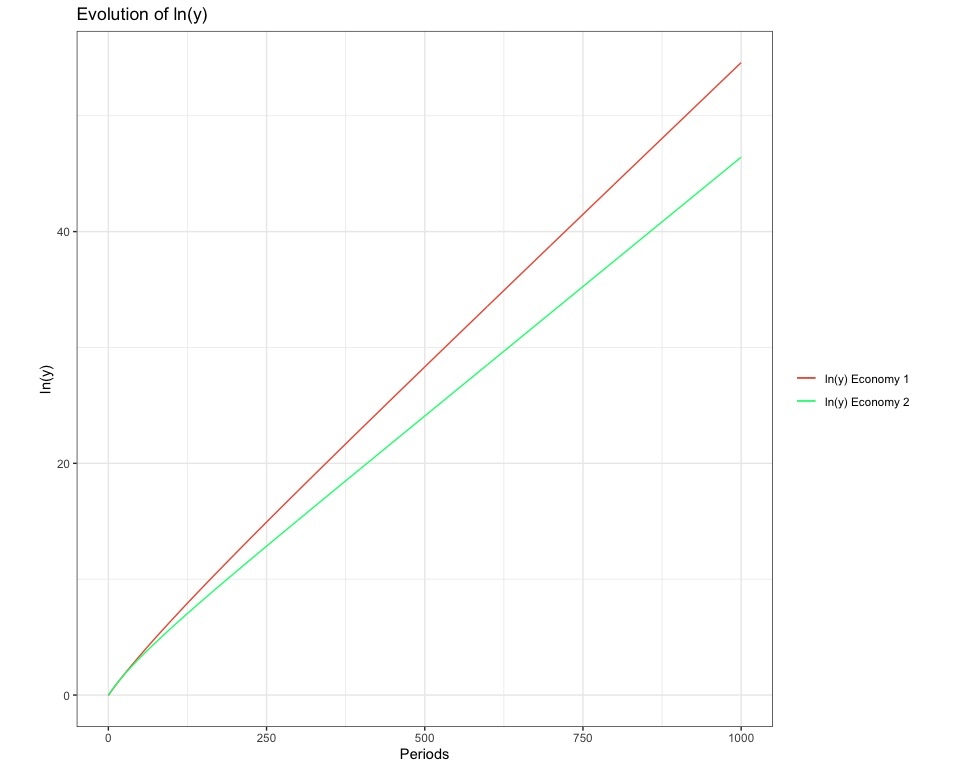
\includegraphics[width=11.5cm]{plots/lny.jpeg}
\end{figure}

\pagebreak
 \begin{figure}[h!]
\caption{$g_t^y$}
\centering
\label{figure2}
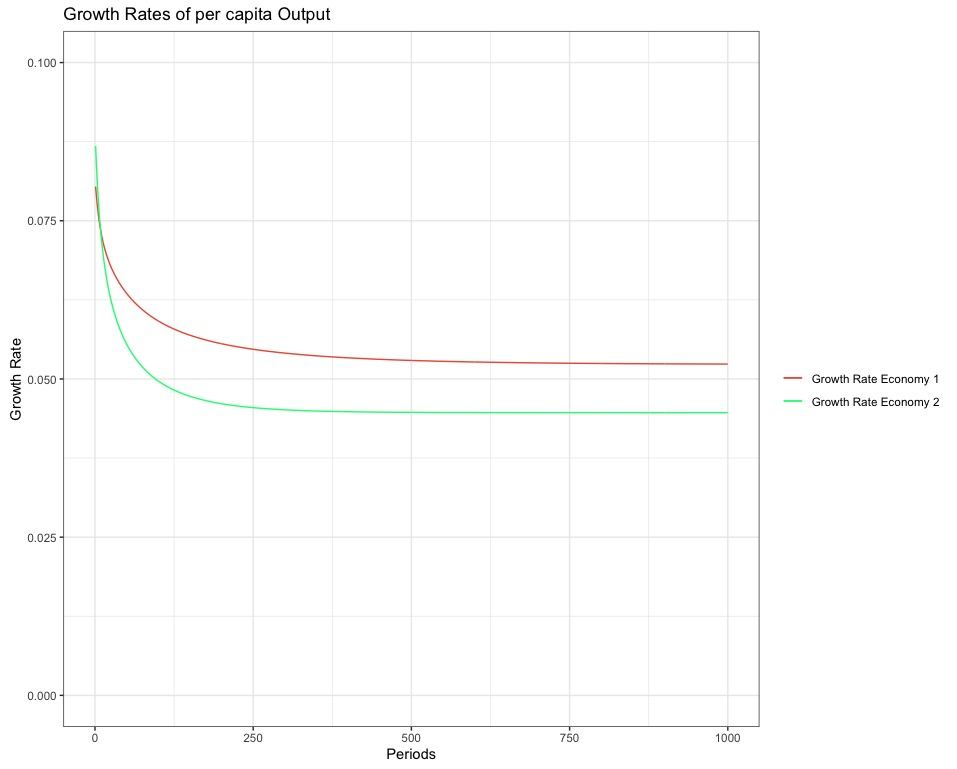
\includegraphics[width=12cm]{plots/percapita.jpeg}
\end{figure}

 \begin{figure}[h!]
\caption{$g_t^y$ and $g_t$}
\centering
\label{figure3}
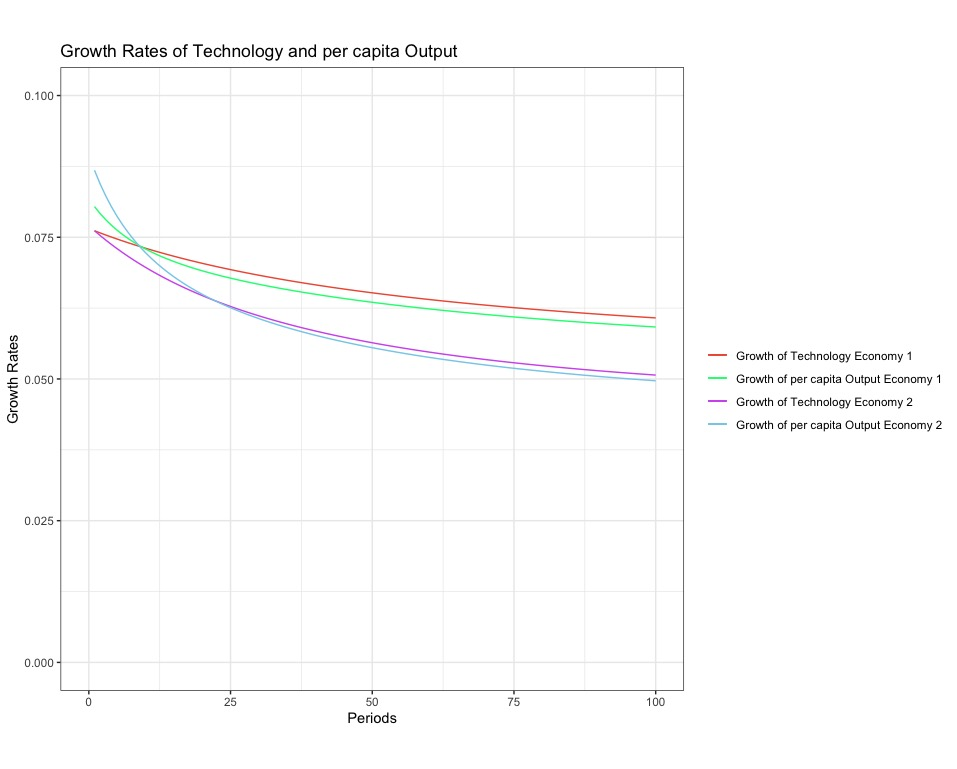
\includegraphics[width=12cm]{plots/comp.jpeg}
\end{figure}



\pagebreak
\textit{d) Discuss your results by comparing the two economies.} \par

In \textbf{Figure 1} one can observe that per capita output increases faster in economy 1 than in economy 2. This can be eplained by the fact that population grows faster in economy 1. Therefore, also the share of labor engaged in R\&D, $L_A$, increases faster. Thus, the growth rate of $A$ is larger in economy 1 which result in higher per capita outputs than in economy 2.\par

\textbf{Figure 2} shows us the growth rate of per capita output. As mentioned before, economy 1 grows faster due to the higher level of technology they acquire. Both economies' growth rates converge to a fixed value after about 500 periods.\par

The last graph, \textbf{Figure 3}, shows the growth rates of technology and per capita output for both economies during the first 100 periods. We can see that the growth rates of technology for both economies start at the same initial point. This makes sense, since the level of technology depends on the amount $L_A$, which is the same in the two economies initially. After that, economy 1 has the advantage, since its population grows faster. As of the growth rate of per capita output, $\Tilde{y}_t$ in economy 2 increases faster than in economy 1 due to the lower growth rate in $A$. Hence, in the beginning where $A$ is similar in both economies, $g_t^y = \ln{y_t}-\ln{y_{t-1}}$ is larger in economy 2, but soon falls below economy 1 as the difference in the level of technology starts to widen.





\pagebreak
\textbf{\Large{Exercise 5.3 - BONUS}}

\textit{Having studied several types of endogenous growth models, summarize the most important features and differences in these models. What drives growth in the semi-endogenous version of these models?}\par 

So far we have studied 3 different endogenous growth models: Externality-Based, R\&D-Based, and Cozzi's model. The first two both have an endogenous and a semi-endogenous case which depend on whether the parameter $\phi$ = 1 or $0 < \phi < 1$.

\par Externality-Based and R\&D-Based models differ in the way they explain technological progress $A_t$. The former assumes productive externalities from capital on labour, that is $A_t = K_t^\phi$. The latter says that a constant share of the labour force $s_R$ works in the R\&D sector to produce "new ideas" and ultimately new technology, that is $A_{t+1} - A_t = \rho A_t^{\phi}L_At^\lambda$, with $L_{At} = s_{R}L_t$. Because of this, some of their state variables and parameters differ, leading to different equations for production functions, law of motion, growth rate of $A_t$, $k_t$ and $y_t$, and steady-state values. One advantage of the R\&D-based model over the Externality-Based is that, while both explain growth, in the former the process is intentional whereas it isn't in the latter.  

\par However in the end, the Externality-Based and R\&D-Based models come to the same conclusions, policy implications, and shortcomings. The semi-endogenous versions suggest policymakers to promote population growth $n$ to increase economic growth, as it is positively correlated with $g_{se}$ in the models, which conflicts with empirical evidence. If convergence towards the steady-state is very slow though, there would be an accordance with transitory growth. Growth in semi-endogenous versions is therefore driven by the population growth rate $n$. The endogenous versions suggest policymakers to enhance savings and investment $s$ to increase economic growth, as it is positively correlated with $g_{se}$ in the models, which is in accordance with empirical evidence. More problematic however is the scale effect the endogenous models imply: a larger constant population results in higher growth, and an increasing population in accelerating growth, making truly endogenous growth implausible. On a side note, in some models where $s_R$ is endogenously defined, it depends positively on $s$, allowing us to make this policy implication for the R\&D-Based model.

\par Even though both models have different focuses regarding policy implications and different views of the innovative process, it is possible to find empirical support of a positive correlation of growth in GDP per capita and savings (in the form of investment) throughout late contemporany history, as well as GDP per capita and population growth, but for specific periods, with the industrial revolution (late nineteenth century and the beginning of the twentieth century) as the most prominent example. So, what if both models are right? This is precisely the motivation for the Cozzi model.

\par As the motivation implies, the Cozzi model tries to join the Truly Endogenous and Semi-Endogenous growth models. That is why it is also called "Hybrid model". The Cozzi model assumes that the "true" model of technological progress is a linear combination of the semi-endogenous and truly endogenous mechanisms, with a parameter $\alpha_{sem}$ to weight both mechanisms. Therefore the major contribution of the Cozzi model is how it express technological growth:

\begin{equation}
    g_t \equiv \frac{A_{t-1}-A_t}{A_t} = \alpha_{sem}\rho{A_t}^{\phi}{L_{A_{t}}}^{\lambda} + (1-\alpha_{sem})\rho{s_{Rt}}^{\lambda}
\end{equation}

\par Thus, manipulating the parameter $\alpha_{sem}$ can influence the kind of technology accumulation we are aiming to have in an economy, which ultimately affects its growth and policy implications cited above.


\end{document}
